\documentclass{report}
\usepackage{geometry}
\usepackage{url}
\usepackage{cite}
\usepackage{graphics}

\title{An Analysis of Security in Bitcoin, a Cryptographic Currency
Implementation}
\author{Ian Dimayuga, Tom Dooner, Will Wettersten \\
\url{{icd3,ted27,wbw20}@case.edu} \\ EECS444
\\ Case Western Reserve University}
\date{April 30, 2012}

\begin{document}
\maketitle
\section*{Cryptographic Currency}
% Tom
Cryptographic currency seeks to solve a timeless problem in economic systems:
how can value be transferred between entities in a way that is fair for both
entities? If the trade is disputed, what value remains with which party? And,
how can value be transferred through an intangible medium?

These are problems that current monetary systems cannot handle. Paper currency
is cumbersome and most-importantly cannot be electronically transferred. The
digital representation of money used by banks is actually just a clever system
of account withdrawals and credits in an agreed-upon order by banks.

\subsection*{Transferring Money, Today}
If an entity wished to transfer money to another entity today, they have a few
choices at their disposal. Some of these options include a check, a wire
transfer, the Automated Clearing House (ACH) system, or
PayPal\cite{wiki:wiretransfer}. All of these methods fail to employ mechanisms
to make them irreversible and impervious to unfair trades.

Wire Transfers rely on sophisticated networks of accounts at various banks, and
unless funds are quickly retrieved from the destination bank, the wire transfer
may be reversed by force of law. Wire transfer fraud is endemic to online
solicitations, and the FBI concludes that wire transfers and ACH transactions
cost businesses \$85 million USD per year\cite{wiretransferssuck}. 

Automated clearing houses are also go-to methods of stealing from unsuspecting
small businesses. The rate of ACH-based attacks on small businesses is growing,
along with the number of lawsuits against the banks that allow these attacks to
happen\cite{achsucks}. New laws place the loss in event of fraud squarely on the
bank. This is an unfortunate legal situation perpetuated by the lack of
technological solutions to the problem of fraud.

\subsection*{Enter Cryptographic Currency}
Cryptographic currency can solve the problem of fraud. If cryptographic currency
can ascribe value to a series of bits, then we can ensure that the appropriate
parties can be confident that their transactions were, in fact, initiated by the
appropriate entities with the right to the money.

However, this imposes new fascinating security problems. How can digital
currency prevent duplicate spending? What security must be taken to maintain the
private keys to your bank balance? Can someone design a system which is
impervious to interference from any single controlling entity?

But most importantly, what properties should digital cash fulfill? To answer
this question, we will take a brief detour into the works of David Chaum.

\section*{Properties of Cryptocurrency}
% Tom
In 1990, David Chaum, cryptologist and mathematician studying at UC Berkeley,
published techniques which allow for the minting of digital
currency.\cite{Chaum:Cash} Blind signature schemes, as they have come to be
called, allow the creation of digital currency which fulfills many desirable
properties of such a cash system. In 1991, Okamoto improved Chaum's algorithm
by identifying these properties of an ideal cryptographic currency and
implementing them:\cite{Okamoto:Cash}

\begin{enumerate}
\item \textbf{Independence}: The electronic cash must not depend on any physical condition.
\item \textbf{Security}: The electronic cash should prevent double-spending and illegal creation.
\item \textbf{Privacy}: Electronic cash transfers should not be traceable by a third party.
\item \textbf{Off-line Payment}: Electronic transfers should be able to occur off-line.
\item \textbf{Transferability}: The cash can be transferred to others.
\item \textbf{Dividability}: The cash can be divided into smaller pieces.
\end{enumerate}

In this paper, we will analyze a specific implementation of electronic cash:
Bitcoin. Bitcoin satisfies these properties, except for off-line payment. We
will specifically focus on Bitcoin's security model and how it has been
relatively error-free over the course of millions of dollars of transactions.

\section*{Introduction to Bitcoin}
% Ian
% Include some graph of Bitcoin usage?

% From http://cryptome.org/0005/bitcoin-who.pdf
%   Talk about Kaminsky's analysis of Bitcoin's Security? (Maybe a subsection to
%    itself?)
%   Talk about the mysterious creator of Bitcoin? (And, how this is perhaps a
%    security benefit for the existence of the program)

\section*{Bitcoin Protocol Security}
% Ian
\subsection*{Creating a Transaction}
\begin{figure}[h]
  \begin{center}
    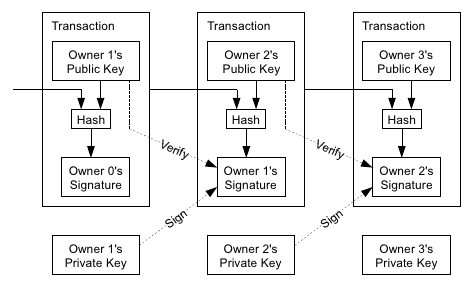
\includegraphics{images/coinchain.png}
    \caption{Satoshi Nakamoto's Bitcoin}
    \label{fig:coinchain}
  \end{center}
\end{figure}
\subsection*{Proof-of-Work Chain}

\section*{Bitcoin Wallet Security}
% Will
Key to the bitcoin network is the bitcoin desktop client.  The client is a desktop
application that users can download to mine and trade bitcoins.  The original client
was released by the creators of bitcoin as an open source c++ project\cite{Andresen:source}, although
subsequent client programs have been released from various third parties.  

A bitcoin user has two seperate goals when protecting their wallet, namely protecting
against wallet loss and protecting against wallet theft.  The the distinction between 
the two is that in the first, a user simply loses access to their wallet by deleting 
the wallet.dat file, losing their computer, or something equally ordinary.  The second 
goal, to protect against wallet theft, is much more complex an issue.

One simple approach to preventing theft that many bitcoin users have taken is actually 
using a paper wallet to store their bitcoing.  Several bitcoin paper wallet utilities 
exist and are free to user on the internet.  To use them, a user typically downloads a 
key generator tool and generates a private key for any number of their bitcoins.  The 
user then prints out the private key and makes sure that it is saved nowhere but 
physically on the piece of paper.  This way, a user can carry around any quantity of 
bitcoins in their physical wallet.  When a user wants, theiy can import the bitcoins 
either to their bitcoin client or to a bitcoin bank like MtGox.

Another simple approach to preventing theft is to encrypt all or parts of the virtual 
wallet.  Many users their wallet.dat file, and the makers of bitcoin are considering 
adding a utility in the next release of bitcoin client that encrypts the private keys 
in the wallet.dat file.  Other users have but their wallet.dat files in encrypted online 
repositories using services like Dropbox or Wuala in conjunction with an encryption 
program like 7-zip or TrueCrypt.  Other users find even more success in encrypting the 
entire directory in which their bitcoin client resides.

Still, however, the Bitcoin wallet represents a serious security problem for Bitcoin.  
By default, the wallet.dat file is not encrypted, so any hacker who can gain entrance 
into a vitims computer can steal their bitcoins simply by copying their wallet.dat file 
and then using then transerring the private keys to their account.  Although not intrinsic 
to Bitcoin theory, the wallet implementation is perhaps the foremost risk to Bitcoin.

\section*{Attacks Against Bitcoin}
% Will

\section*{Conclusion}

\bibliography{security}{}
\bibliographystyle{plain}
\end{document}
